\documentclass[10pt]{standalone}
\usepackage{amsmath}
\usepackage{pgf,tikz}
\usepackage{mathrsfs}
\usetikzlibrary{arrows}
\pagestyle{empty}
\begin{document}
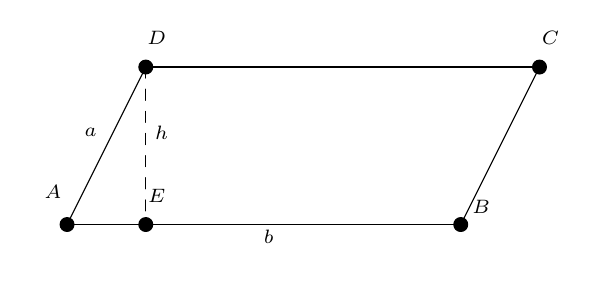
\begin{tikzpicture}[line cap=round,line join=round,>=triangle 45,x=1.0cm,y=1.0cm]
\clip(-2.5,-1.5) rectangle (4.5,1.5);
\draw (-2.,-1.)-- (3.,-1.);
\draw (3.,-1.)-- (4.,1.);
\draw (4.,1.)-- (-1.,1.);
\draw (-1.,1.)-- (-2.,-1.);
\draw [dash pattern=on 4pt off 4pt](-1.,1.)-- (-1.,-1.);
\begin{scriptsize}
\draw [fill=black] (-2.,-1.) circle (2.5pt);
\draw[color=black] (-2.18,-0.59) node {$A$};
\draw [fill=black] (3.,-1.) circle (2.5pt);
\draw[color=black] (3.26,-0.77) node {$B$};
\draw [fill=black] (4.,1.) circle (2.5pt);
\draw[color=black] (4.14,1.37) node {$C$};
\draw [fill=black] (-1.,1.) circle (2.5pt);
\draw[color=black] (-0.86,1.37) node {$D$};
\draw[color=black] (0.56,-1.15) node {$b$};
\draw [fill=black] (-1.,-1.) circle (2.5pt);
\draw[color=black] (-0.86,-0.63) node {$E$};
\draw[color=black] (-0.8,0.17) node {$h$};
\draw[color=black] (-1.7,0.17) node {$a$};
\end{scriptsize}
\end{tikzpicture}
\end{document}